\documentclass[12pt, letterpaper]{article}
\date{\today}
\usepackage[margin=1in]{geometry}
\usepackage{amsmath}
\usepackage{hyperref}
\usepackage{cancel}
\usepackage{amssymb}
\usepackage{fancyhdr}
\usepackage{pgfplots}
\usepackage{booktabs}
\usepackage{pifont}
\usepackage{amsthm,latexsym,amsfonts,graphicx,epsfig,comment}
\pgfplotsset{compat=1.16}
\usepackage{listings}
\lstset{language = python, breaklines=true, basicstyle={\small\ttfamily}}
\usepackage{xcolor}
\usepackage{tikz}
\usetikzlibrary{shapes.geometric}
\usetikzlibrary{arrows.meta,arrows}
\newcommand{\Z}{\mathbb{Z}}
\newcommand{\N}{\mathbb{N}}
\newcommand{\R}{\mathbb{R}}
\newcommand{\Po}{\mathcal{P}}

\author{Alex Valentino}
\title{computational lab 2}
\pagestyle{fancy}
\renewcommand{\headrulewidth}{0pt}
\renewcommand{\footrulewidth}{0pt}
\fancyhf{}
\rhead{
	computational lab 2\\
	292	
}
\lhead{
	Alex Valentino\\
}
\begin{document}
	I did the assignment in python, the code is below:
	\begin{lstlisting}
		import math
import sys

def integrate_riemann(F, t0, t, N):
        accum = 0
        for n in range(N):
                accum += F(t0 + (t-t0)*(n/N))
        return ((t-t0)/N)*accum

def picard(v,x,t0,x0,t,N):
        return x0+integrate_riemann(lambda s: v(x(s),s), t0,t,N)

def search(t,T,high,low):
        if high >= low :
                mid = int((high + low)/2)
                #print(T[mid] <= t)
                #print(T[mid+1] > t)
                #print(mid)
                if(T[mid] <= t):
                        if(T[mid+1] > t):
                                return mid
                        else:
                                return search(t,T,high,mid+1)

                if(T[mid] <= t and T[mid+1] > t):
                        return mid

                if(T[mid] > t):
                        return search(t,T,mid,low)
                else:
                        return search(t,T,high,mid+1)
                return 1

def interpolate(t,T,Y):
        #n = search(t,T,len(T),0)
        n = 0

        l = 0
        u = len(T) - 1
        while(u - l > 1):
                m = (l + u) // 2
                if(t >= m):
                        l = m
                else:
                        u=m

        n = l

        '''
        for i in range(len(T)-1):
                if(T[i] <= t and t < T[i+1]):
                        n = i
                        break
        '''
        if T[n+1]-T[n] == 0:
                print("the issue is " + str(n) +" " +str(T[n]) + " " +str(T[n+1]))
        return Y[n] + (t-T[n])*(Y[n+1]-Y[n])/(T[n+1]-T[n])

def integrate_riemann_interpolated(v,Y,T,t0,t,N):
        accum = 0
        for n in range(N - 1):
                accum += v(interpolate(t0+(t-t0)*n/N,T,Y),t0+(t-t0)*n/N)
        return (t-t0)*accum/N

def picard_interpolated(v,Y,T,t0,x0,N):
        X = []
        for n in range(N + 1):
                X.append(x0 + integrate_riemann_interpolated(v,Y,T,t0,T[n],N))
        return X

def datWrite(file,T,X):
        with open(file, 'w') as f:
                for i in range(len(T)):
                        f.write(str(T[i]) + '\t' + str(X[i]) + '\n')

def main():
        sys.setrecursionlimit(15000)
        # print(integrate_riemann(lambda x:x*x,0,1,1000))
        v = lambda x,t: math.cos(t)*x
        x0 = 1
        t0 = 0
        N = 100
        x1 = lambda t : picard(v,lambda s : 1,t0,x0,t,N)
        print(x1(1))
        x2 = lambda t : picard(v,x1,t0,x0,t,N)
        print(x2(1))
        #x3 = lambda t : picard(v,x2,t0,x0,t,N)
        #print(x3(1))
        #x4 = lambda t : picard(v,x3,t0,x0,t,N)
        #print(x4(1))
#       x5 = lambda t : picard(v,x4,t0,x0,t,N)
#       print(x5(1))

#       T=[2,3,4,5,6]
#       print(search(5.7,T,5,0))
#       print(search(2.5,T,5,0))
        tf = 2*math.pi
        T = []
        for n in range(N+1):
                T.append(t0 + (tf-t0)*n/N)
        print(T)
        X = []
        X1 = []
        X0 = []
        for n in range(N+1):
                X0.append(1)
        X.append(X0)
        for i in range(N + 1):
                X1.append(x1(T[i]))
        print(X1)
        X.append(X1)
        print(len(X))


        for i in range(1,11):
                X.append(picard_interpolated(v,X[i],T,t0,x0,N))
        print(picard_interpolated(v,T,picard_interpolated(v,X[0],T,t0,x0,N),t0,x0,N))
        datWrite("x0.dat",T,X[0])
        datWrite("x5.dat",T,X[5])
        datWrite("x10.dat",T,X[10])

        x1 = lambda t : picard(v,lambda s : 1,t0,x0,t,N)
        N = 1000
        T = []
        for n in range(N+1):
                T.append(t0 + (tf-t0)*n/N)
        X = []
        X1 = []
        X0 = []
        for n in range(N+1):
                X0.append(1)
        X.append(X0)
        for i in range(N + 1):
                X1.append(x1(T[i]))
        #print(X1)
        X.append(X1)
        #print(len(X))


        for i in range(1,11):
                X.append(picard_interpolated(v,X[i],T,t0,x0,N))
        #print(picard_interpolated(v,T,picard_interpolated(v,X[0],T,t0,x0,N),t0,x0,N))
        datWrite("x0D.dat",T,X[0])
        datWrite("x5D.dat",T,X[5])
        datWrite("x10D.dat",T,X[10])
if __name__ == "__main__":
        main()
	\end{lstlisting}
	\begin{enumerate}
		\item First function in the code above.
		\item Second function in the code above.
		\item 
			\begin{itemize}
				\item $x_1 (1) = 1.843762461008662$
				\item $x_2 (1) = 2.1959139982203255$
				\item $x_3 (1) = 2.2935173535489803$
				\item $x_4 (1) = 2.3137216187315204$ 
			\end{itemize}
		\item Fourth function in the code above, there was an attempt to place the time to interpolate into the right bucket recursively to achieve logarithmic performance, but found an easier, functional, implementation off of stack overflow.
		\item Fifth function in the code above.
		\item Sixth function in the code above.
		\item Plotting with $N = 100$\\
		\begin{center}
		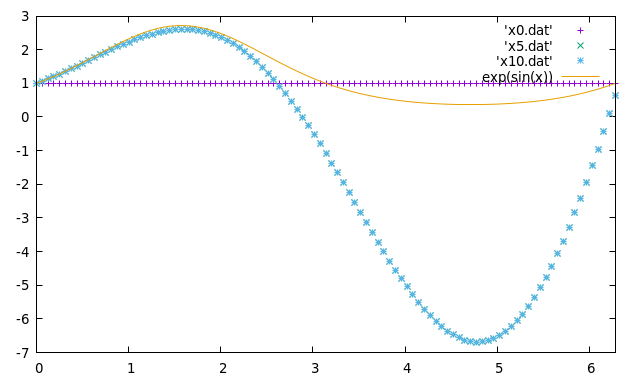
\includegraphics[scale=0.5]{N100interpolatedPicard.png}
		\end{center}
		
		Plotting with $N = 1000$
		\begin{center}
			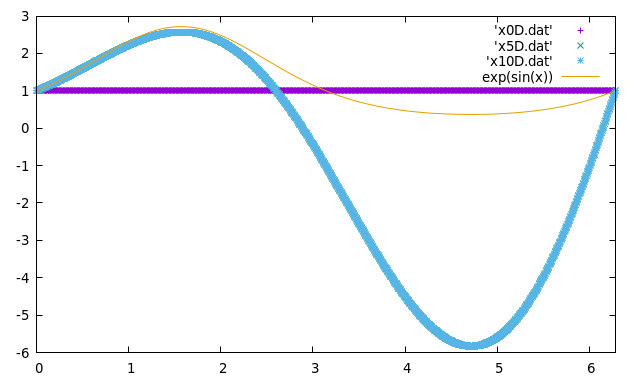
\includegraphics[scale=0.5]{N1000interpolatedPicard.png}		
		\end{center}
		Due to the gnuplot automatically resizing it doesn't pop out but lowest the $N=100$ approximation goes is $\sim-7$ where the $N=1000$ is $\sim-6$
	\end{enumerate}
\end{document}